\scanpage{19}
\mspage{\textcircled{2}}

\textbf{ACADEMIE D'AIX-MARSEILLE}\\
\rule{3cm}{.4pt}\\
\textbf{INSPECTION ACADEMIQUE}\\
\textbf{DE VAUCLUSE}\\
\rule{1cm}{.4pt}

\diagram{\begin{tikzcd}[ampersand replacement=\&,column sep=small,row sep=small]
I\arrow[r,"\text{épi}"]\arrow[dr,"\text{épi}"']\&J\arrow[r,no head]\arrow[dr,no head,bend right]\&{}\\
\&K.\&{}
\end{tikzcd}}
$\operatorname{card} I,J;K\leq3$

\diagram{\begin{tikzcd}[ampersand replacement=\&,column sep=small,row sep=small]
I\arrow[r]\arrow[d]\&J\arrow[r]\arrow[d]\&J'\arrow[d]\\
K\arrow[r]\&\deleted{\unsure{K'}}\arrow[r,no head]\&\bullet
\end{tikzcd}}

\diagram{\begin{tikzcd}[ampersand replacement=\&,column sep=small,row sep=small]
X_0\&X_1\arrow[l]\&X_2\arrow[l]\\
X'_0\arrow[u]\&X'_1\arrow[l]\arrow[u,no head,to path={(\tikztostart.north)--([yshift=-6pt]\tikztotarget.south)..controls([yshift=-2pt]\tikztotarget.south)and([xshift=-5pt,yshift=-2pt]\tikztotarget.south)..([xshift=-5pt,yshift=-5pt]\tikztotarget.south)\tikztonodes}]\&\unsure{X'_2|x'_2}\arrow[l]\arrow[u]
\end{tikzcd}}

\diagram{\begin{tikzcd}[ampersand replacement=\&,column sep=small,row sep=small]
I\arrow[r,hook]\arrow[d]\&J=I\amalg K\arrow[d,no head]\\
I'\arrow[r,hook,no head]\&J'=I'\amalg K
\end{tikzcd}}

\diagram{\begin{tikzcd}[ampersand replacement=\&,column sep=large,row sep=large]
X(I)\&\begin{gathered}\deleted{X(I)\times X(K)}\\
\inserted{X(I\amalg K)}\end{gathered}\arrow[l]\\
X(I')\arrow[u]\&X(I'\amalg K')\arrow[l]\arrow[u,no head,to path={
([yshift=2pt]\tikztostart.north) --
([yshift=-7pt]\tikztotarget.south)
.. controls ([xshift=3pt,yshift=-3pt]\tikztotarget.south)
and ([xshift=-3pt,yshift=-2pt]\tikztotarget.south)
.. ([xshift=-3pt,yshift=-5pt]\tikztotarget.south)\tikztonodes}]
\end{tikzcd}}

\diagram{\begin{tikzcd}[ampersand replacement=\&,column sep=large]
I\arrow[r]\&{}
\end{tikzcd}}

\diagram{\begin{tikzcd}[ampersand replacement=\&,column sep=large,row sep=large]
\mathbb E_n\arrow[r,"{\unsure{\delta|\partial}_n}"]\arrow[d,"K_{n-1}"]\&\mathbb E_{n+1}\\
\mathbb E_n\&{}
\end{tikzcd}}

\deleted{$\unsure{u}$}

\figure{\begin{tikzpicture}
\node at (0,0) {\begin{tikzcd}[ampersand replacement=\&,column sep=small,row sep=small]
\mathbb E_n\arrow[r,"{\unsure{\delta|\partial}_n}"]\arrow[d,"{\unsure{\delta|\partial}_n}"']\&\mathbb E_{n+1}\arrow[d]\\
\mathbb E_{n-1}\arrow[r]\&\mathbb E_{n+2}
\end{tikzcd}};
\node at (2.6,0) {$n\geq1$}; \node at (3.65,.8) {\textcircled{II}};
\node at (0,-2.6) {\begin{tikzcd}[ampersand replacement=\&,column sep=small,row sep=small]
\mathbb E_n\arrow[r,"{\unsure{\delta|\partial}_n}"]\arrow[d,"K_{n-1}"']\&\mathbb E_{n+1}\arrow[d]\\
\mathbb E_{n-1}\arrow[r,to path={(\tikztostart.east)--++(4pt,-2pt)--(\tikztostart.east)--(\tikztotarget.west)\tikztonodes}]\&\mathbb E_n
\end{tikzcd}};
\node at (2.6,-2.6) {$n\geq2$}; \node at (3.65,-2.7) {\textcircled{III}};
\draw (-2,-4)..controls(-1.6,-3.6)and(-1.4,-4.2)..(-1,-3.9)..controls(0,-4.2)and(1,-3.7)..(2,-4)..controls(2.5,-4.2)and(2.8,-3.8)..(3.2,-4);
\node at (0,-5.2) {\begin{tikzcd}[ampersand replacement=\&,column sep=small,row sep=small]
\mathbb E_{n\deleted{\unsure{*}}}\arrow[r,"K_{n-1}"]\arrow[d,"K'_{n-1}"']\&\mathbb E_{n-1}\arrow[d,no head,"{\deleted{\unsure{\alpha}}}"]\\
\mathbb E_{n-1}\arrow[r,no head,"{\deleted{\unsure{\alpha}}}",to path={(\tikztostart.east)--([xshift=-2pt]\tikztotarget.west)--++(0,3pt)\tikztonodes}]\&\mathbb E_{n-2}
\end{tikzcd}};
\node at (2.6,-5.2) {$n\geq3$}; \node at (3.65,-4.8) {\textcircled{IV}};
\node at (0,-7.8) {\begin{tikzcd}[ampersand replacement=\&,column sep=small,row sep=small]
\mathbb E_n\arrow[r,"K_{n-1}"]\arrow[d,"K''_{n-1}"']\&\mathbb E_{n-1}\arrow[d]\\
\mathbb E_{n-1}\arrow[r,no head,to path={(\tikztostart.east) -- ([xshift=-2pt]\tikztotarget.west) -- ++(-4pt,5pt)\tikztonodes}]\&\mathbb E_{n-2}
\end{tikzcd}};
\node at (2.6,-7.8) {$n\geq4$}; \node at (3.65,-7.7) {\textcircled{V}};
\draw (-2.2,.3)..controls(-2.7,2.2)and(2.4,2)..(3.5,.8)..controls(4.3,-1)and(4,-4)..(4.1,-6)..controls(4.4,-8)and(3.9,-9)..(2.8,-9.3);
\end{tikzpicture}}

\figure{\begin{tikzpicture}
\node at (0,0) {\begin{tikzcd}[ampersand replacement=\&,column sep=small,row sep=small]
\mathbb E_p\arrow[d]\&{}\\
\mathbb E_{p\unsure{+}q}\&\mathbb E_q\arrow[l]
\end{tikzcd}};
\node at (.3,1.4) {\textcircled{I}}; \node at (1.8,.6) {$p,q\geq1$};
\draw (-1.7,1.2)..controls(-.2,2)and(2.7,1.8)..(2.7,.2)..controls(2.7,-1.9)and(-.4,-2)..(-1.6,-.8)..controls(-2,-.5)and(-1.9,.2)..(-1.85,.55);
\end{tikzpicture}}

\figure{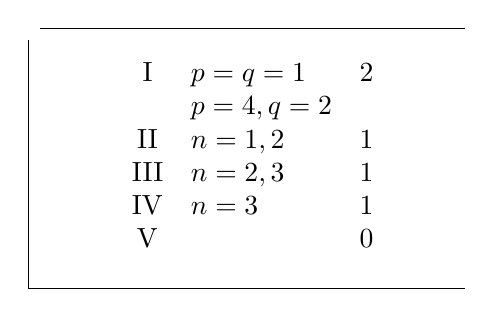
\begin{tikzpicture}
\node[inner sep=8pt] at (0,0) {$\begin{array}{clc}
\mathrm I&p=q=1&2\\
&p=4,q=2&\\
\mathrm {II}&n=1,\deleted{\unsure{2}}&1\\
\mathrm {III}&n=2,\deleted{\unsure{3}}&1\\
\mathrm {IV}&n=3&1\\
\mathrm V&&0
\end{array}$};
\draw (-2.7,1.65)--(2.7,1.65);
\draw (-2.85,1.5)--(-2.85,-1.65)--(2.7,-1.65);
\end{tikzpicture}}

\margin{$\deleted{\unsure{p|*}}$}

\figure{\begin{tikzpicture}[x=.012cm,y=-.012cm]
\node[anchor=west] at (835,1710) {$\mathrm I'$};
\node[anchor=west] at (925,1710) {$p=1,q=3$};
\node[anchor=west] at (925,1760) {$p=2,q=2$};
\node[anchor=west] at (835,1835) {$\mathrm {II}$};
\node[anchor=west] at (925,1835) {$n=2$};
\node[anchor=west] at (835,1902) {$\mathrm {III}$};
\node[anchor=west] at (925,1902) {$n=3$};
\node[anchor=west] at (835,1990) {$\mathrm {IV}$};
\node[anchor=west] at (925,1990) {$n=4$};
\node[anchor=west] at (835,2090) {$\mathrm V$};
\node[anchor=west] at (925,2090) {$n=4$};
\node at (1630,1678) {$2$};
\node at (1630,1810) {$1$};
\node at (1630,1891) {$1$};
\node at (1630,1985) {$1$};
\node at (1630,2080) {$1$};
\draw (810,1660)..controls(825,1800)and(812,2020)..(825,2220);
\draw (835,2180)..controls(1000,2190)and(1140,2145)..(1280,2150)
..controls(1420,2144)and(1530,2145)..(1570,2160);
\node at (1245,1655) {\begin{tikzcd}[ampersand replacement=\&,column sep=large]
\unsure{\mathbb E'}\arrow[r]\&\unsure{\mathbb E'}
\end{tikzcd}};
\node at (1260,1800) {\begin{tikzcd}[ampersand replacement=\&,column sep=large]
{}\arrow[r]\&{}
\end{tikzcd}};

\draw (1395,1795)--(1445,1795);
\draw (1395,1787)--(1395,1803);
\draw (1445,1787)--(1445,1803);
\node at (1465,1712) {$2$};
\node at (1220,1960) {\begin{tikzcd}[ampersand replacement=\&,column sep=small,row sep=large]
\mathbb E^2\&\mathbb E\arrow[l,no head]\\
\mathbb E^{\unsure{\prime|1}}\arrow[u,no head]\arrow[r,equals]\&
\mathbb E^{\unsure{\prime|1}}\arrow[u,no head,"{1}"']
\end{tikzcd}};
\node at (1470,1950) {\begin{tikzcd}[ampersand replacement=\&,column sep=small,row sep=large]
X^2\&X_{\unsure{1}}\arrow[l]\\
X_1\arrow[u]\arrow[r,equals]\&\unsure{X|x}_1\arrow[u,no head,"{1}"',to path={
([xshift=-3pt,yshift=2pt]\tikztostart.north)
.. controls ([xshift=2pt,yshift=1pt]\tikztostart.north)
and ([xshift=1pt,yshift=5pt]\tikztostart.north)
.. ([yshift=8pt]\tikztostart.north)
-- ([yshift=-7pt]\tikztotarget.south)
.. controls ([xshift=3pt,yshift=-3pt]\tikztotarget.south)
and ([xshift=-3pt,yshift=-2pt]\tikztotarget.south)
.. ([xshift=-3pt,yshift=-5pt]\tikztotarget.south)\tikztonodes}]
\end{tikzcd}};

\draw (1175,2143)--(1222,2143);
\draw (1175,2134)--(1175,2153);
\draw (1222,2134)--(1222,2153);
\draw (1286,2150)--(1286,2172);
\draw (1420,2139)--(1420,2168);
\draw (1468,2139)--(1468,2168);
% Cancellation strokes lie over the central diagrams, not over the table's live columns.
\draw[line width=.6pt] (1135,1600)
..controls(1110,1740)and(1090,1900)..(1120,2025)
..controls(1150,2110)and(1190,2110)..(1215,2110);
\draw[line width=.6pt] (1095,1855)--(1295,1600);
\draw[line width=.6pt] (1120,1785)
..controls(1190,1705)and(1245,1600)..(1260,1620)
..controls(1270,1650)and(1180,1835)..(1200,1800)
..controls(1300,1660)and(1395,1620)..(1370,1660);
\draw[line width=.6pt] (1115,2015)
..controls(1235,1860)and(1335,1720)..(1360,1745)
..controls(1380,1775)and(1240,1965)..(1260,1940)
..controls(1350,1840)and(1420,1810)..(1410,1875);
\draw[line width=.6pt] (1150,2080)
..controls(1220,2140)and(1250,1940)..(1290,1910)
..controls(1320,1890)and(1260,2080)..(1285,2070)
..controls(1340,1970)and(1430,1870)..(1420,1965);
\draw[line width=.6pt] (1350,1645)
..controls(1450,1540)and(1365,1790)..(1415,1760)
..controls(1520,1620)and(1475,1750)..(1510,1855);
\draw[line width=.6pt] (1505,1715)
..controls(1495,1870)and(1515,1910)..(1535,1750)
--(1580,2080)--(1495,2150);
\draw[line width=.6pt] (1400,2220)--(1550,1815);
\draw[line width=.6pt] (1230,2090)
..controls(1280,2050)and(1250,2160)..(1300,2145)
..controls(1370,2140)and(1380,2090)..(1420,2110);
\end{tikzpicture}}

\margin{18}
